\chapter{Software Defined Radio}
Software defined radio also known as software radio or SDR is a radio in which
some or all of the physical layer functions are software defined. Due to the  
exponential increase in the ways and means by which people need to communicate
- data communications, voice communications, video communications, broadcast 
messaging, command and control communications, emergency response 
communications and etc, there is a constant need of modifying radio devices 
easily and cost efficiently. The traditional hardware radio system consist a 
variety of analogy elements such as mixers, filters, amplifers, converters, 
modulators and demodulators etc which are costly and are not flexible. Thus 
traditional hardware based radio devices limit cross-functionality and can 
only be modified only through physical intervention. This results in higher 
production costs and minimal flexibility. The solution to this is Software 
Defined Radio which is easily modifiable. Technologies such as Field 
Programmable Gate Array (FPGA), Digital Signal Processor (DSP) and 
General-Purpose Processor (GPP) are used to build the software radio elements.


\begin{figure}
\centering
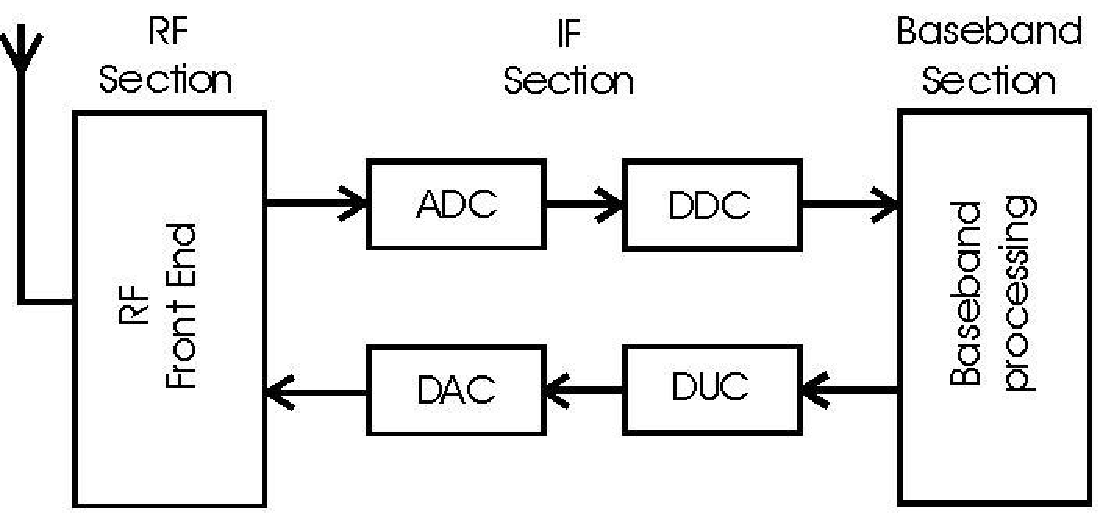
\includegraphics[width=0.59\textwidth]{../images/sdrBlock}
\caption[Block diagram of SDR]{Block diagram of SDR \protect\cite{kranthi13}.}
\label{sdrBlock}
\end{figure}

The software defined radio (SDR) contains a number of basic functional blocks.
The radio in genera can be divided into three basic sections, namely the front
end, the IF section and the base-band section as shown in Figure \ref{sdrBlock}. The 
front end section uses analogue RF circuitry and it is responsible for 
receiving and transmitting the signal at the frequency of operation. IF 
section performs the digital to analog conversion and vice versa. It also 
contains the signal processing like Filtering, modulation and demodulation, 
Digital up conversion (DUC), Digital down conversion (DDC) etc. The last stage
of the radio is the baseband processor. It is at this point that the digital 
data is processed \cite{miller08}\cite{kranthi13}.
We have used GNURadio and USRP N210 to confgure the SDR to implement the
Cognitive Radio test-bed. 

\begin{figure}
\centering
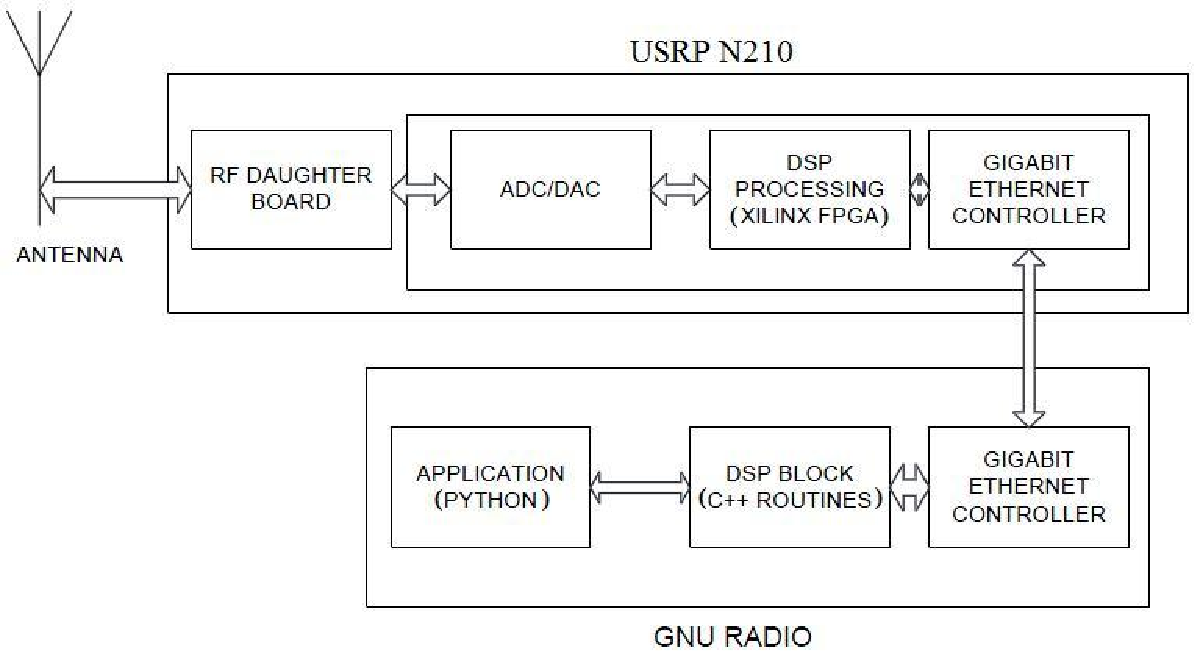
\includegraphics[width=0.59\textwidth]{../images/usrpGNURadioBlock}
\caption[Block diagram for USRP operation with GNURadio]{Block
diagram for USRP operation with GNURadio {\cite{kranthi13}}.}
\label{usrpGNURadioBlock}
\end{figure}

A block diagram of a USRP-based SDR transceiver built with a GNURadio flow 
graph is shown in Figure \ref{usrpGNURadioBlock}. USRP kit is used as a
hardware while GNURadio
package is used for the baseband signal processing tasks. The next sections
describe USRP kits and GNURadio package.

\section{USRP}

The USRP (Universal Software Radio Peripheral) is intended to provide a 
low-cost, high quality hardware platform for software radio. It is designed
and marketed by Ettus Research, LLC. It is commonly used by research labs,
universities, and hobbyists. The USRP platform is designed for RF applications
from DC to 6 GHz. USRPs connect to a host computer through a high-speed USB or
Gigabit Ethernet link, which the host-based software uses to control the USRP
hardware and transmit/receive data.

The USRP Hardware Driver (UHD) is the official driver for all Ettus Research
products. The UHD supports Linux, Mac OS X and Windows.

\begin{figure}
\centering
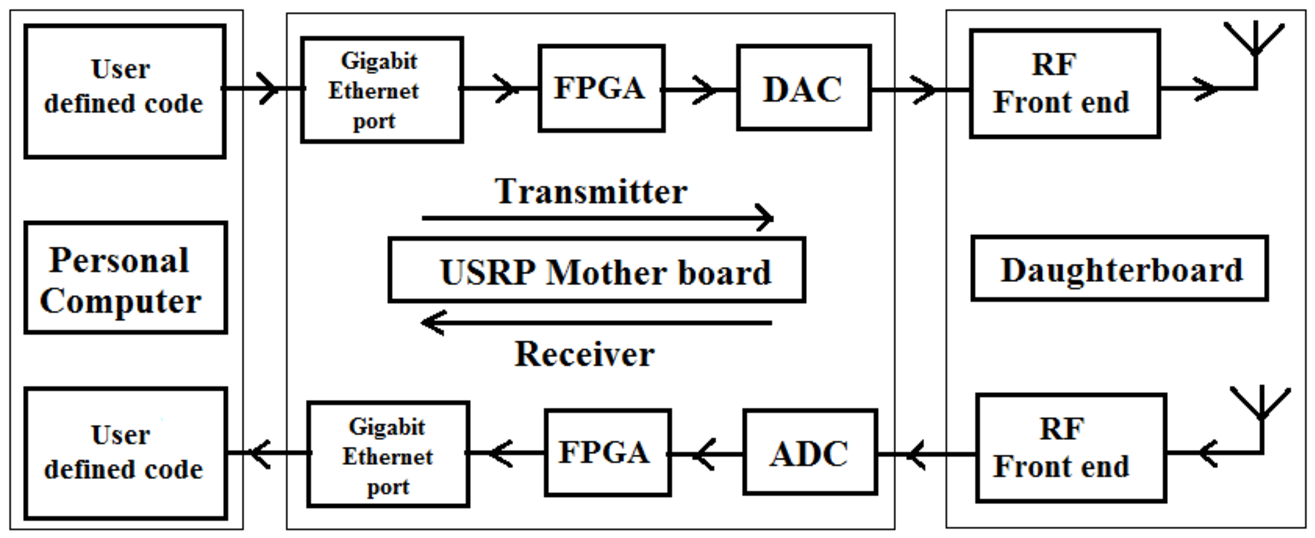
\includegraphics[width=0.7\textwidth]{../images/usrpBlock}
\caption[Block diagram of USRP]{Block diagram of USRP {\cite{kranthi13}}.}
\label{usrpBlock}
\end{figure}

In this project we are using a particular model of USRP product known as the
USRP N210.

\subsection{USRP N210}

The USRP N200 and N210 are the highest performing class of hardware of the 
USRP family of products, which enables engineers to rapidly design and 
implement powerful, flexible software radio systems. The N200 and N210 
hardware is ideally suited for applications requiring high RF performance and
great bandwidth. Such applications include physical layer prototyping, dynamic
spectrum access and cognitive radio, spectrum monitoring, record and playback,
and even networked sensor deployment. The Networked Series products offers 
MIMO capability with high bandwidth and dynamic range. The Gigabit Ethernet
interface serves as the connection between the N200/N210 and the host 
computer. This enables the user to realize 50 MS/s of real-time bandwidth in 
the receive and transmit directions, simultaneously (full duplex).



\section{GNURadio package}

GNURadio is an open source software toolkit for building software defined 
radios. GNURadio is build with the aim to bring the code as close to the
antenna as possible and thereby turn hardware problems into software problems.
GNURadio has software equivalents of real world radio system components like
filters, demodulators, equalizers and other building blocks for signal
processing, as well as a framework for data flow control between them. We can
build a software defined radio by connecting these blocks together. 

\begin{figure}
\centering
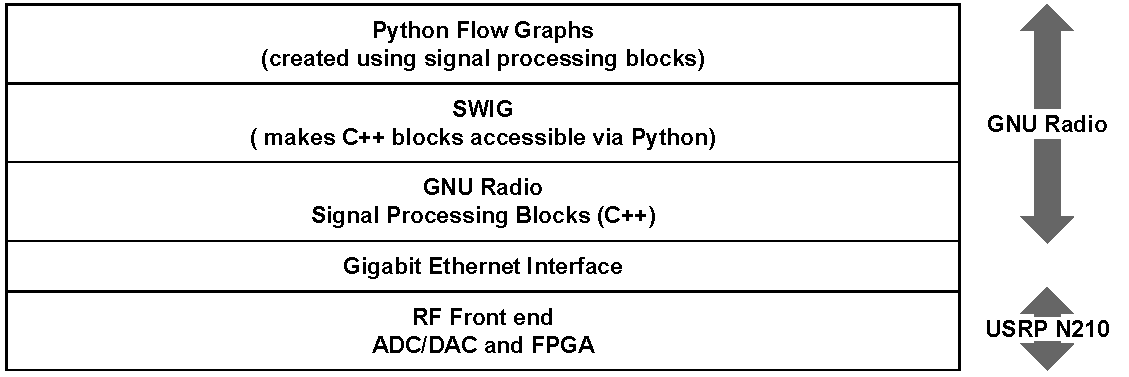
\includegraphics[width=0.9\textwidth]{../images/gnuradio_architecture}
\caption[Architecture of GNU Radio]{Architecture of GNU Radio {\cite{kranthi13}}}
\label{gnuradio_architecture}
\end{figure}

Basically GNURadio does all the signal processing. Functions provided by 
GNURadio includes Mathematical operations, Interleaving, delay blocks, 
Filters, FFT blocks, Automatic Gain Control (AGC) blocks, Modulation and 
demodulation (FM, AM, PSK, QAM, GMSK, OFDM and etc), Interpolation and 
decimation. Apart from signal processing blocks, GNURadio also provides 
support for various signal sources and sinks, such as Signal generators, Noise
generators, Pseudo random number generators, USRP source and sink, Graphical 
sinks, Audio source and sink, File source and sink and etc \cite{wikiGNURadio}.
GNURadio applications are primarily written using the Python programming 
language.

USRP is the hardware used along with GNURadio for SDR and is either at the 
beginning of the flow graph (implementation of a receiver) or the end 
(transmitter).




